% TUGboat class documentation is at:
%   texdoc tugboat
% or
%   https://texdoc.org/serve/tugboat/0
% or
%   https://mirrors.ctan.org/macros/latex/contrib/tugboat/ltubguid.pdf

% guidelines: https://tug.org/TUGboat/location.html

% keep source lines to <= 79 characters
%234567891_234567892_234567893_234567894_234567895_234567896_234567897_23456789

%\DocumentMetadata{
%  lang=en,
%  tagging=on,
%  pdfstandard=ua-2,
%% check-tagging-status,
%  tagging-setup={
%%    math/alt/use,
%    math/setup=mathml-SE
%  }
%}

\RequirePackage{pdfmanagement}
\SetKeys[document/metadata]
{
pdfversion=2.0,
lang=en-US,
xmp=false,
}

\documentclass{ltugboat}
%\usepackage{luatex85}
\usepackage{graphicx}
%\usepackage[all]{xy}
\usepackage{amsmath}
%\usepackage{pgfplots}
\usepackage{microtype}
\usepackage{listings}
\usepackage{booktabs}
\usepackage{tabularx}
\usepackage{array}
\usepackage{siunitx}
\usepackage[hidelinks]{hyperref}

% latexmk could probably do this
\IfFileExists{./tugFigs.pdf}{}{
 \errmessage{Compile local file ./tugFigs.tex first}
}

\lstset{
  columns=fullflexible,
  keepspaces=true,
  commentstyle=\slshape,
  basicstyle=\ttfamily
  \lst@ifdisplaystyle\small\fi,
  language={[LaTeX]TeX}
}

\newcommand{\verbatimOptions}{%
 \IfDocumentMetadataT{setup-code=}\small\makevmeta}

\newcommand{\ltxtalk}{\texttt{ltx-talk}}

\def\url{\tburl}

\title{Creating accessible presentations with \ltxtalk}

% repeat info for each author; comment out items that don't apply.
\author{Timothy Prescott}
\address{University of North Dakota\\101 Cornell Street Stop 8376\\
Grand Forks ND, 58203\\ USA}
\netaddress{timothy dot prescott (at) UND dot edu}
%\personalURL{https://und.edu/directory/timothy.prescott}
\ORCID{0009-0009-0555-8074}

% Electronic access to the article suffices

\begin{document}
\maketitle

%submitted abstract:
%We discuss how to create accessible \PDF\ presentations
%using \ltxtalk, which is similar to \texttt{beamer}.
%We give several examples, including how to adapt common Beamer styles.
%We also discuss necessary adaptations
%to satisfy a common accessibility checker available in several \acro{LMS}s.

\begin{abstract}
We discuss how to create accessible \PDF\ presentations
using \ltxtalk, which is similar to \texttt{beamer}.
We give several examples, including how to adapt common Beamer styles.
We also discuss necessary adaptations
to satisfy a common accessibility checker available in several \acro{LMS}s.
\end{abstract}

\section{Introduction}

In \TUB\ 46:2 \cite{Fischer:2025:NLT}, Fischer and Mittelbach reported that
\begin{quote}
The \texttt{beamer} class is incompatible with the tagging
code and due to the way it is implemented, it is
not easily possible to change this. Joseph Wright
therefore decided to write a new presentation class
called \ltxtalk\ with proper tagging support as a
replacement for \texttt{beamer}.
\end{quote}
I will explore this replacement.

\section{The Basics}

A \ltxtalk\ presentation must begin with
\begin{verbatim}[\verbatimOptions]
\DocumentMetadata{}
\documentclass{ltx-talk}
\end{verbatim}
But we will probably want a \cs{DocumentMetadata} more like
\begin{verbatim}[\verbatimOptions]
\DocumentMetadata{
  lang=en,
  tagging=on,
  pdfstandard=ua-2,
%  check-tagging-status,
  tagging-setup={
%    math/alt/use,
%    role/new-tag=frametitle/H1,
    math/setup=mathml-SE } }
\end{verbatim}
Also, documents must be compiled using \texttt{lualatex} (preferable)
or \texttt{pdflatex}.

The class documentation is available via \texttt{texdoc ltx-talk}
on a command line, or at \url{https://ctan.org/pkg/ltx-talk}.
This links to several examples at
\url{https://www.texdev.net/ltx-talk/examples/}.
If we want to customize the document,
it is important to note that \ltxtalk\ makes use of \emph{templates},
so that we will want to familiarize ourselves
with \texttt{texdoc lttemplates}.

Broadly, we can view a \ltxtalk\ as a properly tagged \LaTeX\ document
that incorporates presentation ideas such as overlays and the geometry.
This means that ``how to'' questions often revolve around
how something should be done in a \LaTeX\ document
or a \texttt{beamer} presentation,
but we will examine several examples that do not fit into those categories.

If we want to define a new overlay aware command,
we should use the \texttt{xparse} syntax
\begin{verbatim}[\verbatimOptions]
\NewDocumentCommand{\mycommand}
  { s D<>{1-} ... }{ ... }
\end{verbatim}
where the \texttt{s} indicates an optional star
(if we want our command to look for that),
the \verb|D<>{1-}| indicates the overlay specification
with a default value \verb|1-|
(or \texttt{d<>} if a default value doesn't make sense),
and then we have whatever other arguments we'd like our function to take.

For example, an upcoming
\begin{verbatim}[\verbatimOptions]
\NewDocumentCommand{\visablealert}{d<> m}{%
  \uncover<#1->{\alert<#1>{#2}}}
\end{verbatim}
creates a new command \cs{visiblealert} that takes
a mandatory overlay specification as \#1 and then a mandatory argument as \#2.
Its content will be covered (transparent) on slides before \#1,
and its content will be alerted on the slide given by \#1.

\ltxtalk\ defines three colors:
alert (red), example (green), and structure (blue).
All three are slightly darker than standard 100\%/0\%/0\%
in \acro{RGB} colors to enhance contrast for accessibility.

If a frame needs to use verbatim or similar to change the catcodes,
then \ltxtalk\ needs a \tubbraced{frame*} environment
(this is similar to \texttt{beamer}'s concept of a \emph{fragile} frame).
As with most things related to verbatim,
such a frame cannot appear as the argument of another command.

\section{Overlays}

\ltxtalk\ modifies many common commands to accept an overlay specification
(after any optional star, but before other arguments),
so that the commands do nothing outside of the specified slides.
\ltxtalk\ also defines the usual overlay commands
\cs{onslide}, \cs{alt}, and \cs{temporal}.
The overlay commands
\cs{alert}, \cs{only}, \cs{uncover}, \cs{visible}, and \cs{invisible}
also have corresponding environments \tubbraced{\meta{action}env}.

These five actions
%(along with \cs{item})
can also combine into \emph{action specifications}:
\cs{item}, \cs{action}, and \tubbraced{actionenv}
allow several actions within one \verb|<...>|.
\meta{action}@\meta{slides} applies the \meta{action} to those slides,
and these are then separated by \texttt{|} within the \texttt{<...>}.

\section{Sections}

Within a frame, the sectioning commands \cs{section}, \cs{subsection}, and
\cs{subsubsection} have no affect.
% Joseph: will there be visible output?
(The other common sectioning commands should not appear in a presentation and
are not defined.)
Outside of the frames, the sectioning commands for sections with frames
contribute to the table of contents, printed by the usual \cs{tableofcontents}.
Before any sectioning command,
this will present an outline of the presentation,
using the usual \texttt{tocdepth} counter to determine
how deep the levels should be displayed
(the default is 2 to display up to \cs{subsection}).
After a sectioning command, this will present the same outline,
but with the non-current sections mostly transparent.

By default, \ltxtalk\ sets frame titles to be \texttt{H4}.
%allowing \cs{section} and similar commands to be above them.
%(\LaTeX\ sets all such sectioning commands as \texttt{H1}.)
The Ally accessibility checker, however,
requires that the heading structure begin at \texttt{H1} and
descend by steps from there.
We can specify that frametitles will be \texttt{H1} by uncommenting
the appropriate line of \cs{DocumentMetadata}.

%* UDOIT ?

\section{Examples}

\subsection{Lists}

Because \ltxtalk\ has adapted the \texttt{beamer}
overlay specification concept, we can still use
\begin{verbatim}[\verbatimOptions]
\begin{itemize}[<+->]
...
\end{itemize}
\end{verbatim}
to create a list that we uncover item by item.
(We generally prefer allowing the audience to take in the entire slide
at their leisure instead of forcing their attention to bounce back and forth,
but recognize that others are allowed to have
their incorrect opinions on the matter.)
If we also want to make use of the more powerful listing environments
created by templates (see \texttt{texdoc blocks-doc}),
then the \verb|<+->| value goes with the key \texttt{action-spec}.
For example,
{\lstset{aboveskip=0pt,belowskip=0pt}
\begin{lstlisting}
\newlength\mylabelwidth
\setlength\mylabelwidth{\widthof{tagged PDFs }}
\begin{frame}
 \frametitle{A Strangely Sporadic Glossary}
\end{lstlisting}
\lstinputlisting{exampleDesc}
\begin{lstlisting}
\end{frame}
\end{lstlisting}}
creates four slides where each item is uncovered in turn,
culminating in \autoref{fig:eg_description}.
\begin{figure}
\setlength{\fboxsep}{0pt}
\fbox{\includegraphics[width=.98\linewidth,page=4]{tugFigs}}
\caption{Output of example \tubbraced{description} code.}
\label{fig:eg_description}
\end{figure}

For tagging purposes, and when creating a printed handout of the slides,
repeating four slides with only slightly varying information
doesn't make sense.
Therefore, only the final slide is represented in those modes.

\subsection{Matrix Multiplication}

As another example, we were able to demonstrate matrix multiplication using
{\lstset{aboveskip=0pt,belowskip=0pt}
\begin{lstlisting}
\begin{frame}[tag-slides=1-]
\frametitle{Matrix Multiplication Example,
 Step \arabic{slide}}
\end{lstlisting}
\lstinputlisting{exampleMatrix}
\begin{lstlisting}
\end{frame}
\end{lstlisting}}
%Because \ltxtalk\ borrows its overlay concepts from \texttt{beamer},
The previous content works in \texttt{beamer} with the only necessary changes
being to remove the \texttt{tag-slides=1-} and
adjust the \cs{arabic}\tubbraced{slide}.
This creates a frame of six slides,
as seen in \autoref{matrixMult}.
\begin{figure}
\setkeys{Gin}{width=.49\linewidth}
\begin{tabular}{|@{}c@{}|@{}c@{}|}\hline
\includegraphics[page=5]{tugFigs}&
\includegraphics[page=6]{tugFigs}\\\hline
\includegraphics[page=7]{tugFigs}&
\includegraphics[page=8]{tugFigs}\\\hline
\includegraphics[page=9]{tugFigs}&
\includegraphics[page=10]{tugFigs}\\\hline
\end{tabular}
\caption{Output of example Matrix Multiplication code.}
\label{matrixMult}
\end{figure}

It is worthwhile to comment on the \texttt{tag-slides=1-} argument.
As we remarked with the previous example,
it is not useful to tag slides with slightly varying information.
Consequently, \ltxtalk\ would normally only tag
the final slide in the frame.
Pedagocically, we would prefer to have \ltxtalk\ tag all slides
in the frame, which is accomplished by the \texttt{1-} specification.
As part of the overlay specifications, \texttt{tag-slides} also recognizes
the variable \texttt{n} as ``the last slide'',
so that the default argument is \texttt{tag-slides=n}.

There is an additional complication if we want
the \texttt{handout} mode of this example (with \texttt{beamer} as well).
By default, the overlay specifications are \emph{flattened},
so that anything that happens on one slide happens on the handout.
This causes the \cs{alert} to apply to all of the items
%(annoying, but fixable)
and the \cs{only} entries to all be visible.

%There are two solutions to this problem.
If we want the handout to follow the \texttt{projector} mode and its tagging,
we can change all of the overlay specifications from \texttt{<\meta{spec}>}
to
\begin{verbatim}[\verbatimOptions]
<projector:!<spec>|handout:!<spec>>
\end{verbatim}
This indicates that the \texttt{handout} specification will follow
the default \texttt{projector} specification.

Alternatively, we can have only the last slide in the handout by using
\begin{verbatim}[\verbatimOptions]
<projector:!<spec>|article>
\end{verbatim}
on non-last slides.

% Joseph may decide this warrants a better syntax
% or that this is a niche enough use case to not bother

\section{Customizations}

\subsection{Adjusting the Header and Footer}

A universal task in presentations is to tailor the header and footer.
These are created in \ltxtalk\ using templates,
which allows convenient customization.
(But we must first remark that these templates are still being developed;
one should consult the documentation if code here does not work as expected.)
The default values of the header template are listed
in \autoref{headerTemplateDefaults}.
\begin{table}
\caption{Default values of the \texttt{header} type \texttt{talk} template}
\label{headerTemplateDefaults}
\centering
\begin{tabular}{ ll }\toprule
Key & Default Value\\\midrule
background-color & (none)\\
color & structure \\
font & \cs{normalfont}\\
height & topmargin (\qty{10}{mm})\\
 & \quad+ headsep (\qty2{mm})\\
left-hspace & leftmargin (\qty{10}{mm})\\
right-hspace & rightmargin (\qty{10}{mm})\\
print-frame-title & true\\\bottomrule
\end{tabular}
\end{table}
We can adjust the values by using
\cs{EditInstance}\tubbraced{header}\tubbraced{std}
\tubbraced{\meta{key=value}}.
Note that the font key is intended for non title elements.
% Joseph? are there non title elements affected by this?
% or is that planned?
Adjusting the font of the title is probably better done with
\cs{EditInstance}\tubbraced{frametitle}\tubbraced{header}
\tubbraced{font=...}.
%\cs{EditInstance}\tubbraced{frametitle}\tubbraced{header}%
%\tubbraced{\meta{key=value}}).

My university encourages a presentation template that has a logo
in the top right of the header.
This cannot be done with the existing template, but can be accomplished with
\begin{lstlisting}
\newsavebox\logobox
\savebox\logobox{%
  \includegraphics[artifact,
    height=\baselineskip]{logofile}}
% possibly after \maketitle frame
\AddToHook{shipout/foreground}{%
  \put(\paperwidth - \wd\logobox - 10mm,
       -8.5mm){\usebox\logobox}} % -\ht\logobox
\end{lstlisting}
%\NewCommandCopy\oldframetitle\frametitle
%\RenewDocumentCommand{\frametitle}{m}{%
%  \oldframetitle{#1\hfill
%    \includegraphics[height=2ex,artifact]
%      {logofile}}}

The default values of the footer template are listed
in \autoref{footerTemplateDefaults}.
\begin{table}
\caption{Default values of the \texttt{footer} type \texttt{talk} template}
\label{footerTemplateDefaults}
\centering
\begin{tabular}{ll}\toprule
Key & Default Value\\\midrule
background-color & (none)\\
color & black \\
element-order & (empty)\\
% author, date, institute, title, subtitle, framenumber, totalframes
font & \cs{tiny}\\
left-hspace & leftmargin (\qty{10}{mm}) \\
right-hspace & rightmargin (\qty{10}{mm}) \\
separator & \cs{hfil}\\\bottomrule
\end{tabular}
\end{table}
The \texttt{element-order} key specifies what information appears
and is a comma separated list of footer-elements
(see \autoref{templatesInstances}), such as
\texttt{element-order=\{title,author,date,framenumber\}}.
The \texttt{totalframes} footer-element displays as an integer.
Outside of the footer, we can access that using
\cs{RefProperty}\tubbraced{lastpage}\tubbraced{totalframes}.

%examples at
%\url{https://www.texdev.net/ltx-talk/examples/}:
%\begin{itemize}
%%\item background-image % as with regular document
%%\item float-centering
%%\item footer-text
%%\item header-footer-color
%%\item list-actions
%%\item list-overlays
%%\item math-fonts % as with regular document
%%\item overlays-opacity
%%\item titlepage-styling
%%\item totalframes
%%\item verbatim-alt-env
%%\item verbatim-content
%%\item actionenv
%\end{itemize}

\subsection{Adjusting the Title Page}

We could
\begin{verbatim}[\verbatimOptions]
\EditTemplateDefaults{titlepage}{talk}
  {!<new key values>}
\end{verbatim}
to adjust the title page, but that is only necessary
if we plan to create multiple title pages.
Instead, we can pass new values as optional arguments to \cs{maketitle},
whose default is equivalent to
\begin{lstlisting}
\maketitle[
  element-order        = {
    title, subtitle, author, institute, date},
  framestyle           = talk,
  horizontal-alignment = center,
  vertical-alignment   = center ]
\end{lstlisting}

%If we have a single title page, we can pass non-default values
%as optional arguments to the \cs{maketitle} command.

The value for \texttt{framestyle} is passed to \cs{pagestyle}.
In addition to the default and \texttt{plain} (no header or footer),
we can also use \texttt{wallpaper} which removes the text
from the footer and the title
(but not their background colors).

\subsection{Creating Custom Elements}

There are two steps to creating a custom element for a title page.
The first is to declare its template instance:
\begin{verbatim}[\verbatimOptions]
\DeclareInstance{titlepage-element}{myelement}
  {talk}{...}
\end{verbatim}
where we use the final argument to change any default template options.
\ltxtalk\ will then use \cs{@myelement},
which we can define with the usual
\begin{verbatim}[\verbatimOptions]
\makeatletter
\newcommand\@myelement{...}
\makeatother
\end{verbatim}

%\subsection{Creating a Custom Footer Element}

Similarly, to creating a custom footer element,
we first declare its template instance:
\begin{verbatim}[\verbatimOptions]
\DeclareInstance{footer-element}{myelement}
  {talk}{...}
\end{verbatim}
\ltxtalk\ will then use \cs{@shortmyelement} or \cs{@myelement}
(favoring the \texttt{short} command if both exist).
If we don't want to change the catcode of \texttt{@},
we can define the desired command with
\begin{verbatim}[\verbatimOptions]
\ExpandArgs{c}\newcommand{@myelement}{...}
\end{verbatim}
For example, we can reproduce the \texttt{beamer} frame counter by using
\begin{lstlisting}
\ExpandArgs{c}\newcommand{@framesoftotal}{%
 \arabic{frame}/%
 \RefProperty{lastpage}{totalframes}}
\end{lstlisting}

\subsection{More Customizations}

The templates and instances created by \ltxtalk\ are
summarized in \autoref{templatesInstances}.
\begin{table}
\caption{Instances and types in the template \texttt{talk} in \ltxtalk}
\label{templatesInstances}
\centering
\begin{tabularx}{\linewidth}{l >{\raggedright} X}\toprule
type & instances \\\midrule
titlepage & \\
titlepage-element & author, date, institute, title, subtitle\\
header & std, wallpaper \\
frametitle & header \\
footer & std, wallpaper \\
footer-element
& date, author, title, subtitle, institute, framenumber, totalframes \\
floatenv & std\\
hidden & std \\
\bottomrule
\end{tabularx}
\end{table}
The \texttt{floatenv} template adjusts the horizontal alignment
of figures and tables using
\begin{verbatim}[\verbatimOptions]
\EditInstance{floatenv}{std}
  {horizontal-alignment = !<alignment>}
\end{verbatim}
where \meta{alignment} is one of left (default), center, or right.
The \texttt{hidden} template adjusts the transparency of hidden items using
\begin{verbatim}[\verbatimOptions]
\EditInstance{hidden}{std}{opacity=!<value>}
\end{verbatim}
where the \meta{value} ranges from 0 (default invisible) to 1 (fully visible).
We may see information about these templates and instances during compilation
and in the log file by using the template commands
\begin{itemize}
\item\cs{ShowTemplateDefaults}\tubbraced{\meta{type}}\tubbraced{talk}
\item\cs{ShowTemplateInterface}\tubbraced{\meta{type}}\tubbraced{talk}
\item\cs{ShowTemplateVariables}\tubbraced{\meta{type}}\tubbraced{talk}
\item\cs{ShowTemplateCode}\tubbraced{\meta{type}}\tubbraced{talk}
\item\cs{ShowInstanceValues}\tubbraced{\meta{type}}\tubbraced{\meta{instance}}
\end{itemize}

% Joseph
\section{Future Work}

As \ltxtalk's reason for existence is proper tagging,
please let us know of any tagging difficulties that you find.

We are intensely interested in feedback from screen reader users
(as opposed to automated validators)
as to what heading structure is useful to them.
Such users are encouraged to get in contact with us.
On a related note, we also would appreciate feedback about requested
\cs{frametitle} customizations.

%We recommend using \cs{begin}\tubbraced{verbatim}\texttt{[\textbackslash small] ...}
%\cs{end}\tubbraced{verbatim} for code blocks, since we prefer not to

%\section{References}
%
%For references to other issues of \TUB, please use the format
%\textsl{volno}:\textsl{issno}, e.g., ``\TUB\ 32:1''.

%The primary \TUB\ style documentation is the \texttt{ltubguid} manual,
%available online at \tbsurl{ctan.org/pkg/tugboat} or locally with
%\texttt{texdoc tugboat}. For general \CTAN\ package references, we
%recommend that form, using \texttt{/pkg/}. If you need to refer to a
%specific file on \CTAN, use:\\
%\texttt{https://mirror.ctan.org/\textsl{path}}

%We recommend using \BibTeX\ (but don't require it), with the
%\texttt{tugboat} \BibTeX\ style. The \texttt{biblio} directory on \CTAN,
%\tbsurl{ctan.org/pkg/biblio}, provides files \texttt{tugboat.bib} with a
%complete bibliography of \TUB, \texttt{texbook3.bib} with many common
%\TeX-related books and articles, and plenty more.

%Email \verb|tugboat@tug.org| with any questions.

\bibliographystyle{tugboat} % tugboat's bibtex style
%\nocite{book-minimal}       % make the example bibliography non-empty
\bibliography{references,tugboat}
%\bibliography{xampl}        % xampl.bib comes with bibtex

\makesignature
\end{document}
